% small note for reference on the "design":
% we've established that minesweeper is NP-complete, that moves have individual difficulty and reward, and that RAC can be used to find move difficulty.
% We're interested in human-percieved difficulty, so instead of looking at playthroughs made by machines, we look at playthroughs made by players.
% we will prove that this is viable for recreating time to solve, and will state that future work should generate playthroughs in a human-like fashion to allow time prediction without humans actually playing. there is a lot of possible specialisation in this, e.g. by taking into account a human's learned techniques from past playthroughs.

As we've explored, the effective difficulty of a Minesweeper field as experienced by the player is very complex, with many contributing factors including actual logical complexity, player skill, and pathfinding (extende with luck as well) to name a few.
This section summarises the background and distils it into a over-arching model that tries to account for all the contributing factors explored so far that can affect the end-to-end difficulty when a human is solving a Minesweeper field.

\subsection{logical-complexity and player-skill balance} \label{awa:challengeSkillBallenceMonolith}
\todoPi{This section explains the tie between complexity and player skill, using paper evidence. This honestly belongs in the background I think, but it also concentrates the information into our model representation, which is part of our design. again a conflict where info should be separated, but I idk how to without removing the necessary context.}

% actual logical complexity has already been well-researched

\todoB{VVVVVVVVVVVVV}
As is covered across many articles of research such as those by \cite{skillChallengeBalance, skillChallengeBalanceAgain, SkillIssueTbh}, generally, logical complexity and player skill are two sides of the same coin which can be balanced to create the feeling of "flow".

\citet{skillChallengeBalanceAgain}outlines very specific conditions for flow state, which are generally met during Minesweeper gameplay,
but two conditions specifically are relevant for consideration here: 1. there is a balance between a user's perception of their skills and the offered challenge, and 2. the offered challenge is clear and unambiguous.


In Minesweeper (and most other CSP games), players are allowed to control the subject of their own attention and are fairly unconstrained.
Beyond the primary goal of field completion, players alter their behaviour in whatever way possible to optimise for solve time (the specific aim of "time" being primarily supported by \citet{skillChallengeBalance}).
\todoB{$\uparrow\uparrow\uparrow\uparrow\uparrow\uparrow\uparrow\uparrow\uparrow\uparrow\uparrow$}
\todoBA{VVVVVVVVVVVVVVV}
There are many ways a player could alter their behaviour such as their tendency to go for easy moves, their threshold for time sunk into a portion of a board before deviation, the tolerance for when to fall to a random guess, and ultimately their frustration level before ending the game and/or moving to a different field (to name a few).

Players adapt their behaviour in accordance with the aforementioned flow, which they optimise in an effort to achieve their best solve time.

The behavioural patterns mentioned above can be boiled down to the player asking themselves "where should I go" in response to "this place is not worth it".
We suggest that the logical complexity, player skill, and navigational factors relevant in this thought process is sufficient to explain the end-to-end difficulty experienced by a player.
However, because it is such a broad definition, this project cant reasonably test all such contributing factors in their entirety.
Instead, since the logical aspect is already very well-researched, we will focus on the human skill aspect and eventually suggest future work that could account for field exploration.
(\todo{note to self: this will be exhaustive enumeration of paths for non-determinism, and pattern-specific logging for a further improvement to the human aspect.})
\todoBA{$\uparrow\uparrow\uparrow\uparrow\uparrow\uparrow\uparrow\uparrow\uparrow\uparrow\uparrow$}

\todoOr{VVVVVVVVVVVVVVV}
Player skill is entirely defined by the player's abilities. We do not have any method to directly learn the player's abilities,
however we do have ways to directly measure a field's difficulty.
As a workaround, we can observe how players behave upon encountering mine arrangements of different difficulties, and use this instead as a test of skill.

For this purpose, we need a correct measure for the difficulty of a mine arrangement, and subsequently a collection of mine arrangements of varying difficulty.

While sourcing an exhaustive list of minesweeper techniques for use when analysing a Minesweeper playthrough would be helpful, such a list may be impossible to construct.
Minesweeper patterns are not restricted to simply the 8 neighbours of a cell. Patterns are formed from different neighbour combinations across multiple cells, and can span the whole board in some cases such as \ref{fig:longPattern}. Since patterns are so unconstrained, a collection of every pattern may boil down to a naive collection of every possible assignment of mines to a field.

Instead of trying to identify every different type of move made, we can use the aforementioned Relational Arc Consistency (RAC) algorithm, which can be repeatedly applied while progressively increasing parameters, to identify the number of constraints that had to be considered for the move to be possible. This groups moves according to their logical complexity, and lets us look at minesweeper moves in a purer form.
\todoOr{$\uparrow\uparrow\uparrow\uparrow\uparrow\uparrow\uparrow\uparrow\uparrow\uparrow\uparrow$}

% NOTE to self: this is, by definition, conjecture. it's 3 hours before teh deadline, so nothing can be done now, but you should fix it when you review this.
\subsection{Relating Humans Applying Minesweeper Techniques to Constraint Propagation (useful? pending rewrite)} \label{awa:theHumanPlayingPipeline}
\todo{distill maybe?}
\todoPi{this basically explains the human playing process, and relates it to pathfinding. it's kind-of more of what I said above, but thought-out from start to finish from a player's perspective}
% In the similar CSP problem of sudoku, \citet{sudokuComputationalModel} proposes that constraint propagation is not only more efficient than backtracking search, it is the natural approach humans take for constraint satisfaction problems. Their research does not directly address this claim, but it vaguely supports it and it is reasonable to expect this behaviour to appear in our findings as well.

\todoB{VVVVVVVVVVVVVVVVVVVVVV} \\
\todoPl{in this lil blue section, I'm basically explaining how RAC corresppnds to minesweeper techniques. I didnt realise that's what I was doing when I was writing it.. anyways: it should be moved to the paper that introduces the link between minesweeper techniques and RAC.}
As previously explored by \citet{sudokuComputationalModel}'s sudoku research, human CSP solving vaguely follows a particular protocol for how they apply their knowledge to play a game. Humans first start with the easiest techniques they are aware of, for example in minesweeper looking at "corner" cells (as illustrated in \cref{fig:cornerexample}) or any other cell where the number of hidden neighbours equals the number of indicated mines, i.e. techniques that only need one level of consistency to identify.

Second to this, when there are no more such instances the player can find within their area of focus, they fall to the next type of difficulty for the techniques they apply. In minesweeper, the next level of consistency includes patterns such as 1221 arrangements (shown in \cref{fig:1221example}) against a wall of closed cells, a case that tells the player there are 2 mines next to each other exactly parallel to the double 2s. Another such pattern is a 121 sequence against a wall, which indicates there is a single mine directly contacting each 1, and an empty cell contacting the 2. This pattern requires 2-consistency to identify because it is not identifiable from a single constraint stemming from a single open cell. In the 121 case, the presence of the 2 asserts there are 3 possible combination of mines: either both on the left, both on the right, or both at either end. The solver is not able to determine which of these cases are the correct arrangement, without noticing that the leftmost 1 rules out the possibilities of 2 mines being on the left, because that would mean 2 mines are present in the jurisdiction of a 1 which would not be consistent with 1 mine being in it's neighbourhood. the symmetric case on the other side with the other 1 eliminates the case where there are 2 cells on the rightmost side, leaving the only possibility /where there is 2 mines on either side of the 2's area. This pattern and others of similar complexity or harder are documented by \citet{msPatterns}.

\begin{figure}[htbp]
    \begin{subfigure}{0.21\textwidth}
        \centering
        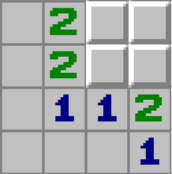
\includegraphics[height=2cm]{embeddables/easycornerSmallV2.png}
        \caption{Easy corner pattern}
        \label{fig:cornerexample}
    \end{subfigure}
    \begin{subfigure}{0.21\textwidth}
        \centering
        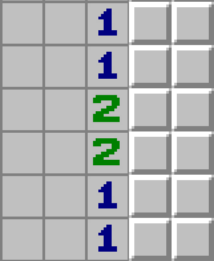
\includegraphics[height=2cm]{embeddables/1221smallV2.png}
        \caption{Slightly hard 1221 pattern}
        \label{fig:1221example}
    \end{subfigure}
    \caption{Minesweeper patterns of different difficulty}
    \label{fig:basicPatterns}
\end{figure}

After a human's known patterns are exhausted on a portion of the board, they may then fall back to their typical approach using constraint propagation to discern new patterns, where the player must enumerate possible states and progressively reduce them down to a reasonable solution. Alternatively, if the player has no known patterns whatsoever, they may also immediately go into this approach, a behaviour that's been observed by \citet{humanCSPapproach} on participants approaching unseen CSP challenges.
\todoB{$\uparrow\uparrow\uparrow\uparrow\uparrow\uparrow\uparrow\uparrow\uparrow\uparrow\uparrow$}

\subsection{human navigation of the minesweeper playing field} \label{awa:pathfindingWRTgameLogicStructure}
\todoPi{this is also pathfinding I think. Further, it's pathfinding in terms of the underlying structure of the complexity of the field (i.e. w.r.t. "clusters" as is defined by Cicvarek)}
what does it mean to be a "perfect" minesweeper player? \\
"imperfect" playing stems from the human nature to deviate on difficult portions of the board.. making "perfection" then means to remove the need to deviate, by augmenting the player/solver with the knowledge necessary.
\todoR{but what about the most basic path to take? even if you know every possible move, you still need to choose which of the possible moves to use, and where to go} \\

As a symptom of minesweeper's nature (\todoR{<-- what makes minesweeper a navigable game, and others not?}), playing a large enough game with an appropriate mine density can give rise to "clusters". These are defined, as by \citet{minesweeperGameGridGeneration}, to be groups of cells, where each constraint on each cell operates on other cells, who are also part of this cluster, i.e. there is no logical "connection" between clusters.

Thanks to this game structure, players can and do deviate from their current path very frequently as they approach moves they have not learned or cant apply easily.

In fact, \citet{whyArePuzzlesFun} (on a similar NP-complete puzzle game, Sokoban) considers this "deviation" to be fairly complex and highly varied from person to person or skillset to skillset, and worth researching. \todo{flesh out}

To understand the reasoning for this, we consider a typical minesweeper playthrough. A playthrough starts somewhere on the board with a random guess, and players continue randomly guessing until they strike a cell with a hint 0, which subsequently triggers the auto-reveal feature of Minesweeper \citet{minesweeperAutoreveal}.

Besides random guesses, there is in fact a more strategic guessing strategy. \citet{Studholme2001MinesweeperCSPencoding} suggests that, if the goal is to find a cell with a hint of 0, then it's most optimal to pick the cell with the least neighbours. The reasoning comes from the probability of a cell being empty, which is itself given by the probability of a single neighbour containing a mine, raised to the power of the number of neighbours. Since the probability of a neighbour containing a mine is between 0 and 1, the probability of the chosen cell having a neighbour with a mine can only decrease as neighbours increases.

Regardless of guessing strategy, the auto-revealed cells upon finding a 0-hint cell is then (usually) enough information for the player to start applying logical reasoning, learned heuristics, etc.

Among the newly revealed cells, the player can now either keep guessing to find more 0-hints (a technique used for an extra early boost in competitive play \todo{cite}) or start deciding on the next move according to the currently available information.

Deciding, then, can be informed by several strategies (these being listed in order of prerequisite experience needed):
the simplest but most inefficient strategy (beyond guessing) is simple brute-force.
assigning flags to various positions, and checking that their assignment holds within the wider context of the board (solving for consistency). \todo{citation for this}

second to this, possible moves can be identified by heuristics, patterns learned by the player from previous gameplay that can allow them to shortcut brute force enumeration and make a decision sooner.
\\
$\uparrow$ there is a great deal of nuance at this stage, depending on the player's experience. less experienced players with less learned patterns may identify less possible moves, and be more "starved" and hence gravitate strongly to the only moves they know.
Conversely, more experienced players with a more accessible playing field, have more choice in where they move.

This leads on to the next move decision strategy, "pathfinding".
Pathfinding refers to how the player navigates the aforementioned minesweeper clusters (something inexperienced players cant do, as they dont have the skill to "break in to" a cluster of difficult moves) and setting themselves up via move "entropy", the measure of how much information a given cell provides to the player upon making the move. On top of picking the closest move to minimise mechanical limits, advanced players may sacrifice a closer move for a further one, with more "entropy", because it gives more progress on the board overall.

\subsection{field pathfinding, or "luck"} \label{awa:pathfindingCompromiseWithHumans}
\todoPi{this section is about the navigational/pathfinding stuff mentioned in sec 3 "project design". specifically, how I sidestep it to allow the experiment to only focus on player skill without needing to consider pathfinding. it SHOULD NOT further refine the idea of pathfinding at all... the problem is that it does, because I've not refactored it. where should I move it? } \\
\todoPi{it also introduces "steppings stones" for pathfinding, explaining people-found paths as a compromise for full path enumeration}
\todo{actually, this section is unnecessarily verbose I think..} \\
% \todoLg{also this section} \\
\subsubsection{the design part}
we will outline the different ways people could deviate, 


\subsubsection{the implementation part}
to consider the typical difficulty for a minesweeper field, you of course need to consider the typical path.

theoretically, people arent necessary for this.
you may use a machine to enumerate every possible path,
and then draw conclusions on the field difficulty from that.

however, this is in practice of course very difficult because, for a 3bv value $x$ of (e.g. 40), there are $x$ different moves that all have to be made at one point or another. two different paths all have the same moves, just in a different order, hence there are $x!$ (e.g. $40! = 8.1591528 \cdot 10 ^{47}$) different possible field paths.

One may think that there is no practical need to enumerate every such path, and indeed that is correct.
consider the minesweeper pattern shown in \cref{fig:1221example}. The player can use logic to determine there are two discernible mines,
each being to the left of each of the twos shown. the player can subsequently deduce the square immediately north of the two mines is safe, and also that the square immediately south is safe.
The player can reveal the north square and then the south square, or the south square and then the north square.
alternatively, the player could only reveal the north square, and then proceed with the information they obtained from the north square, leaving the south square for later (this case also being mirrored).

Going for the north square is equivalent (within one move) to going for the south square, provided only that the player immediately goes for the south square afterwards.
Going for the north square and then proceeding elsewhere is NOT equivalent (within one move), and similarly going for the south square and proceeding elsewhere is also not equivalent.
This is given that we're considering equivalence over one move. all paths are eventually equivalent over the length of the playthough (provided it ends in a win)
\\ \\
The paths I've presented are only subtly different in the grand scheme of the playing field, and can be treated as practically equivalent as far as perceived difficulty is concerned.
\\ \\
Paths which are not perceptually equivalent, are paths which reveal different types of information earlier or later.
In the example, I glossed over picking the north cell and then deviating elsewhere (and the symmetric case) because I explain it now.
suppose the north cell contains a 1. In that case, the player is able to make deductions on the three west-most neighbours.
in such a case, the southern cell could be similarly easy, or be harder.

This gives rise to a complete guess, where the correct guess will lead to better performance, and the incorrect guess would not.

To make an effective difficulty metric, one would need to consider the average difficulty across all paths,
taking advantage of paths whose difficulty are practically equivalent and merging them in enumeration to cut down on the search space,
but still accounting for both paths in the computed average.
$\uparrow$ while still making sure not to merge different paths.

That may be done by checking practical equivalence within a distance of one move,
however this is just a heuristic and I suspect there's more to consider.